% !TeX spellcheck = nl_NL
%%=============================================================================
%% Methodologie
%%=============================================================================

\chapter{\IfLanguageName{dutch}{Methodologie}{Methodology}}
\label{ch:methodologie}

%% TODO: Hoe ben je te werk gegaan? Verdeel je onderzoek in grote fasen, en
%% licht in elke fase toe welke stappen je gevolgd hebt. Verantwoord waarom je
%% op deze manier te werk gegaan bent. Je moet kunnen aantonen dat je de best
%% mogelijke manier toegepast hebt om een antwoord te vinden op de
%% onderzoeksvraag.
Om het effect van zowel K8s ``best-practice'' als K8s security tools op een cluster te onderzoeken werd er gekozen om het onderzoek in 3 scenario's onder te verdelen. Met als doel gegevens te verzamelen over enkele criteria, namelijk het resource gebruik, de stabiliteit en de opstarttijd van de cluster. Voordat we aan de scenario's kunnen beginnen, worden eerst nog alle stappen doorlopen voor het opzetten van de cluster. Nadat de cluster opgezet is zullen we beginnen met het eerste scenario namelijk het opzetten van een basis cluster om de functionaliteit van K8s aan te tonen en om baseline gegevens te verzamelen voor het onderzoek. Deze cluster zal dienen als basis om verdere scenario's verder uit te werken. Als tweede worden er enkele ``best-practice'' gehanteerd bij het opzetten en de configuratie van de cluster, dit om te onderzoeken wat voor effect deze hebben op de cluster. Ten slotte zal er bij het opzetten en configureren van de cluster gebruik gemaakt worden van enkele K8s security tools, dit om te testen wat deze precies doen en wat voor effect deze kunnen hebben op de criteria. 

Gedurende dit onderzoek werd er gebruik gemaakt van de volgende hardware en software:

\begin{itemize}
	\item Besturingssysteem: Pop!\_OS 20.10 x86\_64
	\item Host systeem: MSI GL62 7REX
	\item Kernel: 5.11.0-7614-generic (Linux)
	\item Cloud provider: Linode\footnote{cloud.linode.com/}
	\item Nodes: 3 X Linode 2GB (1CPU core, 2GB RAM, 50GB opslag)
\end{itemize}

\section{Opzetten van de Kubernetes cluster}
In dit hoofdstuk zal de basis cluster opgezet worden. Deze manier van werken zal ook gebruikt worden om de andere scenario's uit te voeren.

Voor het opzetten van de cluster zijn er maar drie onderdelen nodig. 
\begin{itemize}
	\item Account bij een cloud provider, in dit geval Linode.
	\item Kubectl om de cluster besturen.
	\item De Docker image om een applicatie te deployen op de cluster.
\end{itemize}

Aangezien Kubectl op zowel Linux, Windows als MacOS kan draaien, en de cluster zelf bij de cloud provider wordt gehost kunnen deze scenario's op bijna elke computer worden nagebootst. De stappen in volgende hoofdstukken worden allemaal uitgevoerd op een Linux systeem en kunnen dus verschillen op Windows of MacOS. Het is ook aangeraden om een nieuwe directory aan te maken zodat alle bestanden op eenzelfde plaats te vinden zijn.

Voor dit onderzoek zal gebruik gemaakt worden van de ingebouwde ``Linode Kubernetes Engine''(LKE). Deze installeert automatisch de correcte onderdelen op de verschillende worker nodes en creëert ook een gratis master node. Hiervoor werd gekozen omdat het volledig opzetten van een K8s cluster niet binnen de scope van dit onderzoek ligt. Door gebruik te maken van de LKE kunnen we ons dus focussen op de security van de cluster. 

\subsection{Linode Kubernetes cluster}
In dit hoofdstuk zullen de verschillende stappen die doorlopen zijn bij het opzetten van een Linode K8s cluster beschreven worden.

Voor het creëren van een cluster in Linode hebben we enkel een Linode account nodig. Het aanmaken van de cluster zelf is zeer gemakkelijk en gebeurt via cloud.linode.com > Kubernetes > Create Cluster. Vul dan de naam, regio en versie van de cluster in zoals in figuur \ref{fig:LinodeNaam}.

\begin{figure}[h]
	\centering
	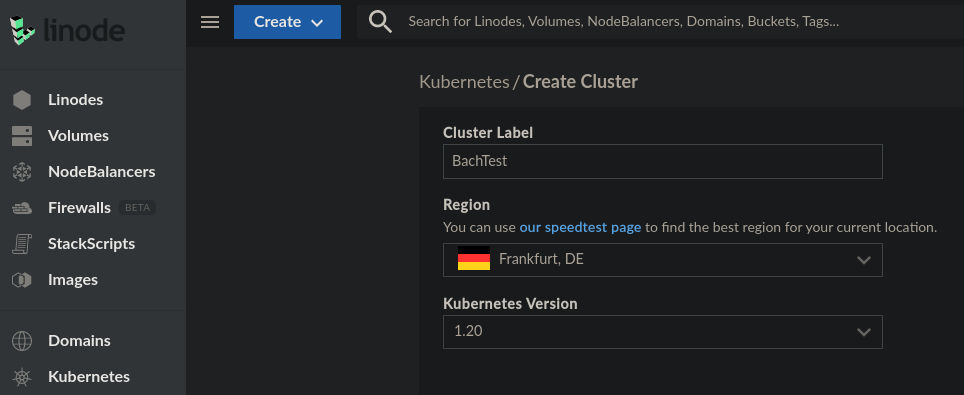
\includegraphics[width=\linewidth]{img/LinodeClusterNaam.png}
	\caption{Aanmaken Linode cluster}
	\label{fig:LinodeNaam}
\end{figure}

Vervolgens kunnen we nodes toevoegen aan de cluster. Voor dit onderzoek gaan we een kleinschalige cluster opzetten met drie worker nodes en één master node. In figuur \ref{fig:LinodeAddNodes} zijn de verschillende soorten nodes die we kunnen toevoegen opgelijst. Tijdens deze scenario's zal gebruik gemaakt worden van drie ``Linode 2GB'' nodes. Daarnaast is het ook mogelijk om nodes van verschillende grotes in dezelfde cluster toe te voegen. De master node is niet meegerekend in deze drie nodes maar word door Linode gratis aangeboden bij het opzetten van een K8s cluster.

\begin{figure}[h]
	\centering
	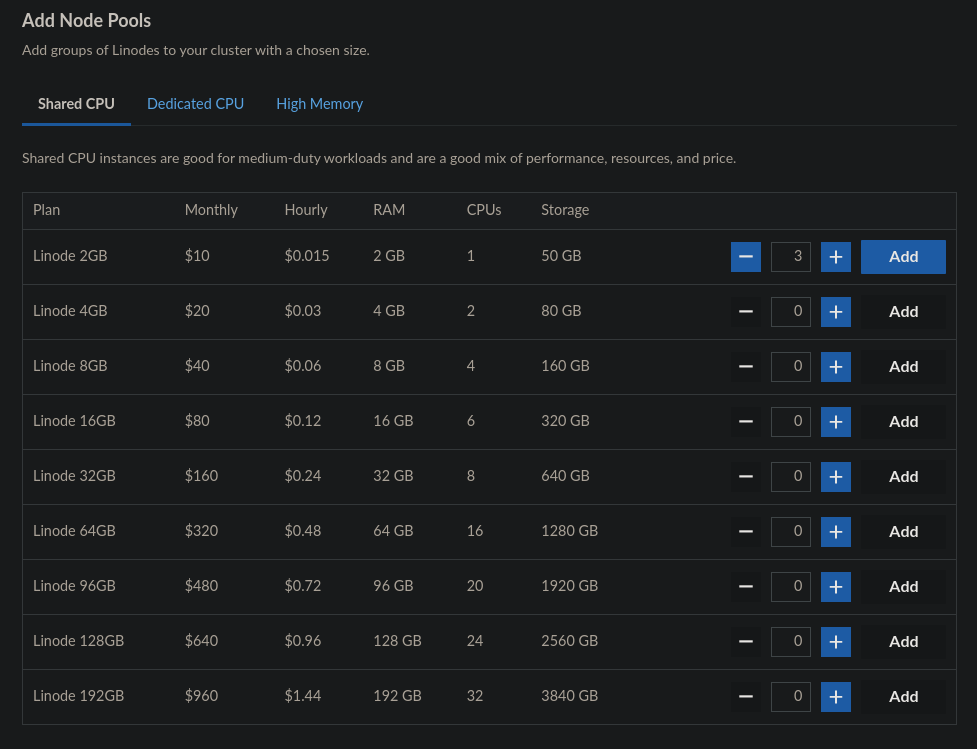
\includegraphics[width=\linewidth]{img/LinodeAddNodes.png}
	\caption{Toevoegen van nodes aan cluster}
	\label{fig:LinodeAddNodes}
\end{figure}

Als alle nodes zijn toegevoegd wordt de cluster aangemaakt. Linode zal hierbij in de achtergrond de gekozen nodes aanmaken alsook de master node klaarmaken voor gebruik. 

Eenmaal de cluster is aangemaakt en opgestart is moeten we deze nog configureren. Deze configuratie gebeurt via Kubectl in volgende stappen.

Als eerste moeten we het kubeconfig.yaml bestand downloaden van Linode. In dit bestand staan alle nodig details om te Kubectl te connecteren met onze cluster. De kubeconfig van de net aangemaakte cluster is te zien in figuur \ref{kubeconfig} (enkele waarden werden ingekort om de leesbaarheid te vergroten).

\begin{figure}[h] 
	\inputminted[fontsize=\footnotesize,linenos]{yaml}{files/BachTest-kubeconfig.yaml}
	\caption{kubeconfig.yaml}
	\label{kubeconfig}
\end{figure}

Vervolgens moet het pad naar het bestand geëxporteerd worden naar de omgevingsvariabele ``KUBECONFIG'' met het volgende commando:
\begin{minted}{bash}
$ export KUBECONFIG=<pad naar file>/kubeconfig.yaml
\end{minted}

We kunnen testen of dit gelukt is door het volgende commando uit te voeren. Dit zou de drie aangemaakte nodes in onze cluster moeten teruggeven.
\begin{minted}{bash}
$ kubectl get nodes
NAME                          STATUS   ROLES    AGE    VERSION
lke25332-32960-608682818f2e   Ready    <none>   6d4h   v1.20.5
lke25332-32960-60868281f030   Ready    <none>   6d4h   v1.20.5
lke25332-32960-608682824efd   Ready    <none>   6d4h   v1.20.5
\end{minted}

Nu Kubectl in contact staat met de ``kube-apiserver'' dewelke op de master node staat, kunnen we beginnen met het configureren van onze cluster. Dit kan zowel met ``ad-hoc'' commando's als met zogenaamde deployments die werken via het ``principle of desired state''. Met andere woorden specificeren de deployments de verschillende  aspecten van de cluster waarbij K8s ervoor zorgen dat aan deze specificaties voldaan worden.

Een deployment is eigenlijk niets anders dan een YAML bestand waarin beschreven wordt hoe de cluster er moet gaan uitzien. Via het volgende commando wordt een deployment op een cluster gezet.
\begin{minted}{bash}
$ kubectl apply -f deployment.yaml
\end{minted}

\subsection{Resetten van cluster}
Na het uitvoeren van elk scenario zal de cluster weer worden gereset zodat het vorige scenario geen impact kan hebben op de rest van het onderzoek. Het resetten van de cluster bestaat vooral uit het verwijderen van deployments en services. Het verwijderen van een deployment wordt gedaan aan de hand van volgend commando.
\begin{minted}{bash}
$ kubectl delete deployment <Deployment naam>
\end{minted}
Het verwijderen van een service verloopt op dezelfde manier.
\begin{minted}{bash}
$ kubectl delete service <Service naam>
\end{minted}
	
\subsection{Gegevens- verzameling en verwerking}
Om conclusies te kunnen trekken uit dit onderzoek hebben we gegevens nodig. Meer bepaald gegevens over de bovengenoemde criteria, namelijk het resource gebruik, de stabiliteit en de opstarttijd van de cluster. Deze gegevens zullen gebruikt worden om de onderzoeksvraag ``Welke impact hebben \textit{best practices} en \textit{security tools} op de criteria?'' te beantwoorden. De verzameling van deze gegevens zal gebeuren via \textit{sysstat}\footnote{github.com/sysstat/sysstat}. Dit is open source tool die ons in staat stelt om een hele hoop verschillende soorten data van ons systeem te exporteren naar bruikbare formaten (zoals JSON, CSV en XML). Deze bestanden kunnen we dan later in RStudio gebruiken om er statistische modellen mee te maken. Sysstat zal op een van de nodes in de cluster worden geïnstalleerd door een ssh verbinding op te zetten en dan volgend commando uit te voeren.
\begin{minted}{bash} 
$ sudo apt-get install sysstat
\end{minted}

Vervolgens moeten we de data collectie aanzetten door in het bestand \verb|/etc/default/sysstat| de variabele \verb|ENABLED| van\textit{''false''} naar \textit{''true''} om te zetten. Vanaf nu zal een van de meegeleverde tools, namelijk sar, elke 10 minuten een nieuwe entry maken in het bestand \verb|/var/log/sysstat/sa<dag van de maand>|. We kunnen deze bestanden uitlezen met behulp van het \verb|sar| commando. Om het CPU gebruik van het systeem om te zetten naar een csv bestand, het het later in RStudio te verwerken, kunnen we het volgende commando gebruiken. In figuur \ref{CPUDataPreview} is het net gecreeerde csv bestand te zien.

\begin{minted}{bash} 
$ sar -f /var/log/sysstat/sa08 >> /root/CpuGebruikDag8.csv
\end{minted}

\begin{figure}[h]
	\centering
	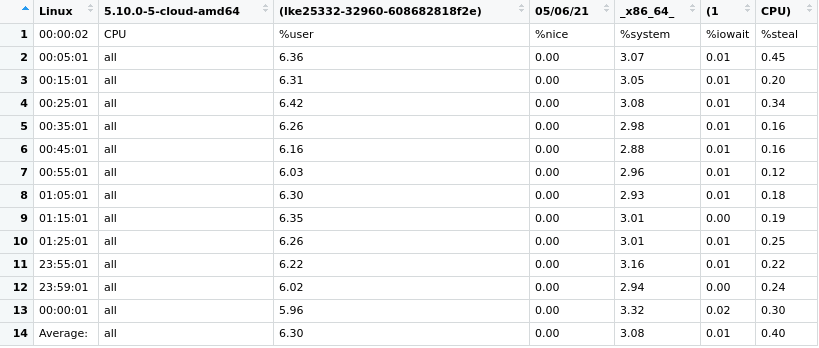
\includegraphics[width=\linewidth]{img/CPUDataPreview.png}
	\caption{Klein deel van het gebruikte csv bestand}
	\label{fig:CPUDataPreview}
\end{figure}

Vervolgens kunnen we door andere \textit{flags} mee te geven aan het sar commando verschillende soorten data uit de logbestanden halen. Het RAM gebruik kan bijvoorbeeld met volgend commando in een csv bestand worden opgeslagen.

\begin{minted}{bash} 
$ sar -f /var/log/sysstat/sa08 -r >> /root/RAMGebruikDag8.csv
\end{minted}

Als laatste moeten de gegevens lokaal op de computer beschikbaar zijn. Dit wordt gedaan door een SFTP verbinding te maken met de node waar sysstat op geïnstalleerd is en de volgende commando's uit te voeren. 

\begin{minted}{bash} 
$ sftp root@172.105.86.96
root@172.105.86.96 s password:
Connected to 172.105.86.96.
sftp> lcd /home/nick/Desktop
sftp> get CpuGebruikDag8.csv
Fetching /root/CpuGebruikDag8.csv to CpuGebruikDag8.csv
\end{minted}

Nu alle nodige gegevens zijn verzamelt kan er begonnen worden aan het verwerken van deze gegevens. Dit wordt gedaan door gebruik te maken van R en Rstudio. 

Het eerste criteria is het vergelijken van het gemiddeld resource gebruik van zowel de CPU als het RAM geheugen. Dit kan simpelweg door de laatste rij van het csv bestand af te lezen. Hier wordt door sar automatisch het gemiddelde berekent. 

Het tweede criteria is de stabiliteit van het systeem. Dit zal onderzocht worden door een Boxplot te maken op basis van de verzamelde gegevens om de hoeveelheid routiers visueel voor te stellen. De R code om dit te doen voor het CPU gebruik staat in figuur \ref{CPUBox}. In dit R script wordt het csv bestand eerst ingelezen zonder de eerste rij omdat deze niet nuttig is voor het verdere onderzoek. Vervolgens nemen we enkel de achtste kolom over omdat hier de hoeveelheid ongebruikte CPU kracht staat. Deze wordt dan afgetrokken van honderd om zo tot de gebruikte hoeveelheid CPU te komen. Als laatste wordt de naam van kolom veranderd zodat het gemakkelijker is om deze te gebruiken bij het maken van de boxplot. De laatste lijnen van het script zijn verantwoordelijk voor het creëren en opmaken van de boxplot. Een voorbeeld van de bekomen boxplot is te zien in figuur \ref{fig:CPUBoxEx}.

\begin{figure}[h] 
	\inputminted[fontsize=\footnotesize,linenos]{R}{files/dataCpuBox.R}
	\caption{R code om boxplot van CPU gegevens te bekomen}
	\label{CPUBox}
\end{figure}

\begin{figure}[h]
	\centering
	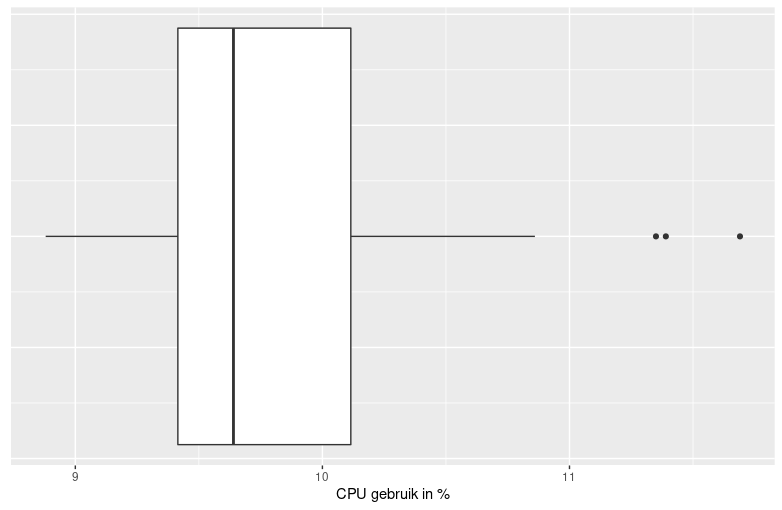
\includegraphics[width=\linewidth]{img/CPUBoxEx.png}
	\caption{Voorbeeld boxplot CPU data}
	\label{fig:CPUBoxEx}
\end{figure}

Voor de gegevens van het RAM gebruik wordt op dezelfde manier te werk gegaan. De R code om de gegevens met betrekking tot het RAM geheugen wordt beschreven in figuur 
\begin{figure}[h] 
	\inputminted[fontsize=\footnotesize,linenos]{R}{files/dataRAMBox.R}
	\caption{R code om boxplot van CPU gegevens te bekomen}
	\label{CPUBox}
\end{figure}


Het algemene resource gebruik van de cluster kan ook voorgesteld worden als een gewone grafiek waarin het resourcegebruik van zowel de CPU als het RAM geheugen worden voorgesteld ten opzichte van de tijd. Het R script om dit te bekomen staat in figuur \ref{CPUGraph}. Een voorbeeld van een bekomen grafiek is te zien in figuur \ref{fig:CPUgraphEx}
\begin{figure}[h] 
	\inputminted[fontsize=\footnotesize,linenos]{R}{files/dataCpuGraph.R}
	\caption{R code om grafiek van CPU gegevens te bekomen}
	\label{CPUGraph}
\end{figure}

\begin{figure}[h]
	\centering
	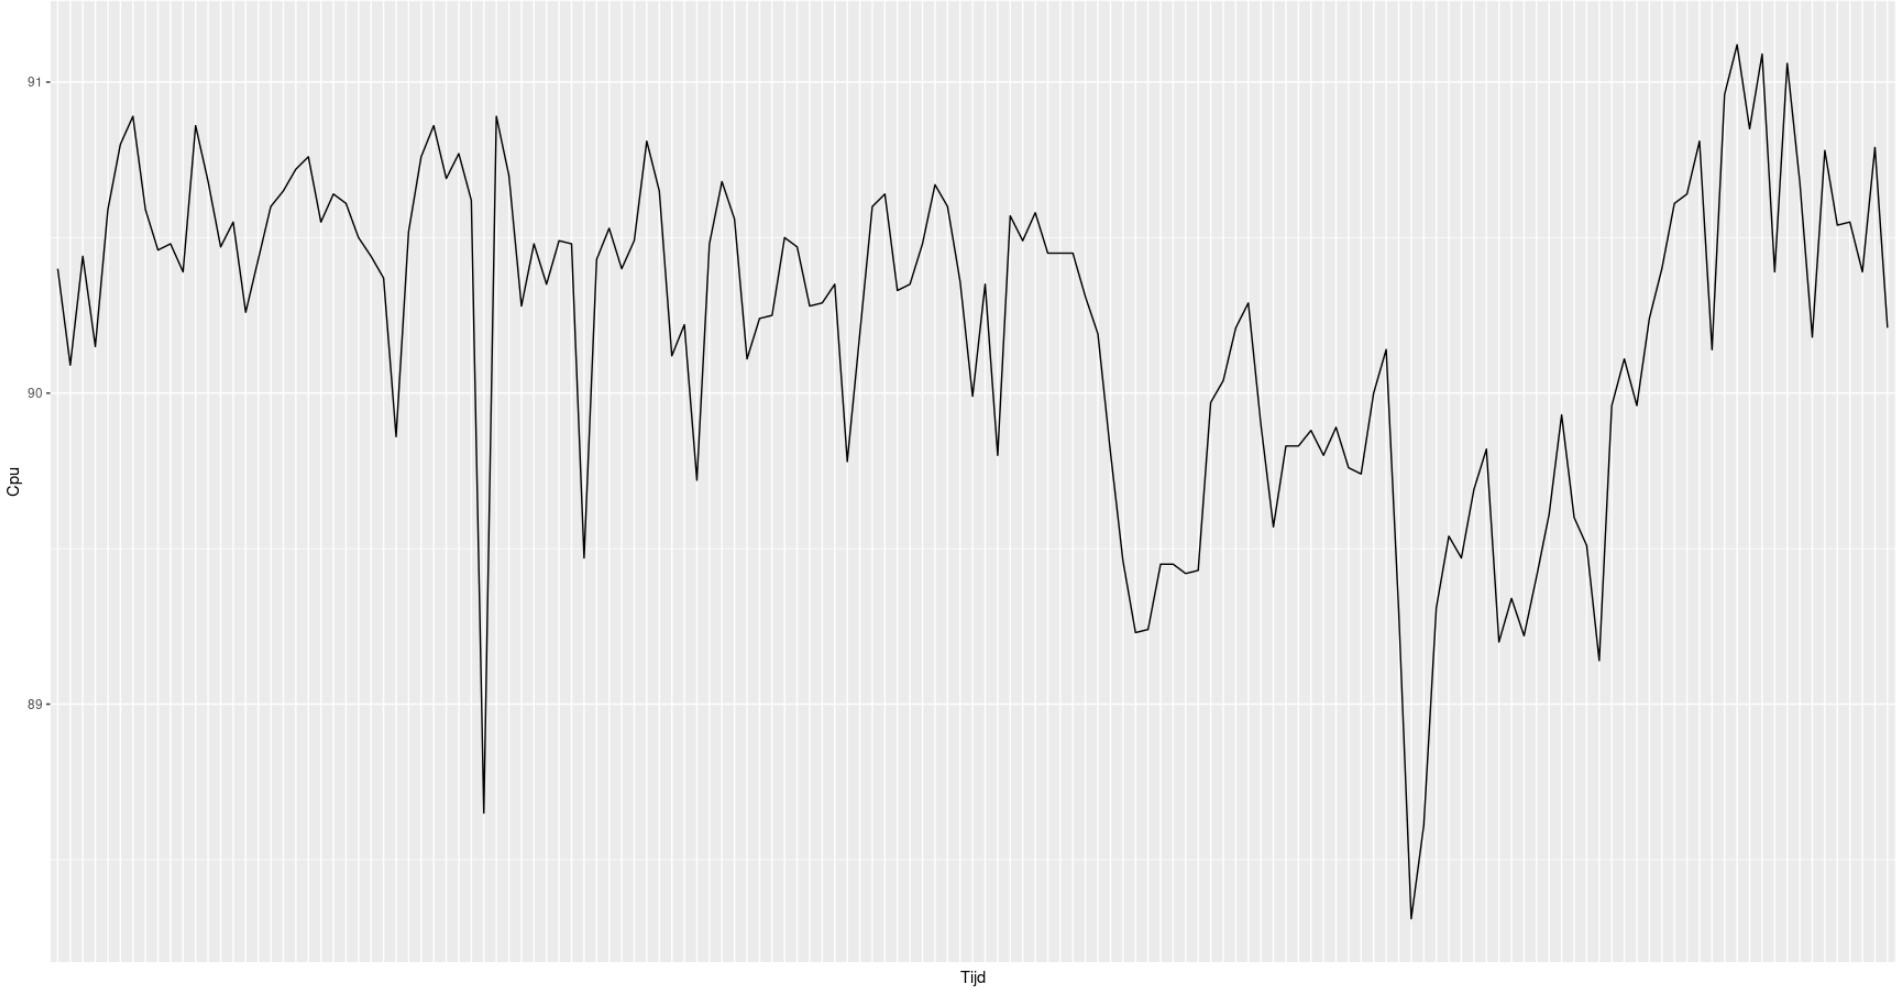
\includegraphics[width=\linewidth]{img/CPUGraphEx.png}
	\caption{Voorbeeld grafiek CPU data}
	\label{fig:CPUgraphEx}
\end{figure}

\clearpage
\section{Scenario 1: Cluster opstelling zonder oog voor security}
\begin{itemize}
	\item Basic deployment van een statische website uitleggen aan de hand van commando's, screenshots en config files. 
	\item deployment YAML tonen en deels uitleggen
	\item Service YAML tonen en deels uitleggen
	\item Nodige gegevens uit de cluster halen met sysstat
	\item Verzamelde gegevens verwerken met RStudio en grafieken/statistieken tonen en uitleggen.
\end{itemize}

%Het eerste scenario bestaat eruit om een simpele cluster op te zetten zonder specifiek oog te hebben voor de beveiliging. De deployment die zal gebruikt worden wordt in figuur \ref{basicDeploy} weergegeven. Hierin wordt een simpele demo website opgezet door gebruik te maken van de image \verb|thenetworkchuck/nccoffee:pourover|. Het aantal pods dat wordt gecreëerd wordt bepaald door de waarde van de \verb| replicas| variabele, in dit geval worden er 3 pods gecreëerd. Er wordt aangeraden om in een productieomgeving het aantal pods en nodes ongeveer gelijk te houden. De variabele \verb|imagePullPolicy: Always| zorgt ervoor dat de Docker image telkens moet worden gedownload van de registry, ook al is deze locaal aanwezig. 
Het eerste scenario bestaat eruit om een simpele cluster op te zetten zonder specifiek oog te hebben voor de beveiliging. De deployment die zal gebruikt worden wordt in figuur \ref{basicDeploy} weergegeven. Enkele van de variabelen worden hieronder uitgelegt: 
\begin{itemize}
	\item \verb|image: thenetworkchuck/nccoffee:pourover|: Dit is de Docker image met de statische demo site.
	\item \verb|replicas:3|: Het aantal pods die moeten worden gecreëerd wordt door deze variabele ingesteld. In dit geval zijn dat er 3 omdat er wordt aangeraden om in een productieomgeving het aantal pods en nodes ongeveer gelijk te houden.
	\item \verb|imagePullPolicy: Always|: Deze variabele zorgt er in dit scenario voor dat de Docker image steeds word gedownload uit de registry als de deployment wordt gebruikt.
	\item \verb|containerPort: 80|: Dit zorgt ervoor dat de site via poort 80 beschikbaar zal zijn.
\end{itemize}

\begin{figure}[h] 
	\centering
	\inputminted[fontsize=\footnotesize,linenos]{yaml}{files/deployment.yaml}
	\caption{deployment.yaml}
	\label{basicDeploy}
\end{figure}

Als de deployment YAML bestand klaar is kan deze met volgend commando op de cluster zetten.
\begin{minted}{bash} 
$ kubectl apply -f deployment.yaml
\end{minted}
Het opzetten van de pods kan gevolgt worden met het volgende commando. In figuur \ref{fig:getPodsDeployment1} is te zien hoe de pods een voor een klaargemaakt worden.
\begin{minted}{bash} 
$ kubectl get pods
\end{minted}

\begin{figure}[h]
	\centering
	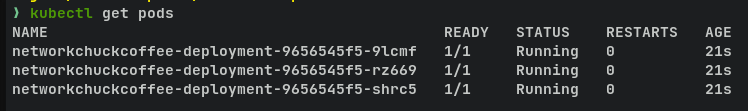
\includegraphics[width=\linewidth]{img/kubectlGetPodsDeployment1.png}
	\caption{Pods worden klaargemaakt}
	\label{fig:getPodsDeployment1}
\end{figure}

Als we nu de deployment willen aanpassen zonder de cluster volledig af te breken kunnen we het commando 
\begin{minted}{bash} 
$ kubectl edit deployments networkchuckcoffee-deployment
\end{minted}
gebruiken. In figuur \ref{editDeploy1} is de output van dit commando te zien. Als we in dit bestand bijvoorbeeld de \verb|replicas| variabele zouden aanpassen en het bestand opstaan, zal K8s merken dat er iets is veranderd. Omdat er gebruik wordt gemaakt van het ``Principle of desired state'' zal er automatisch aan de nieuwe specificaties worden voldaan. Om dit aan te tonen zal de variabele veranderd worden van drie naar vijf.

%\begin{figure}[ht]
%	\centering
%	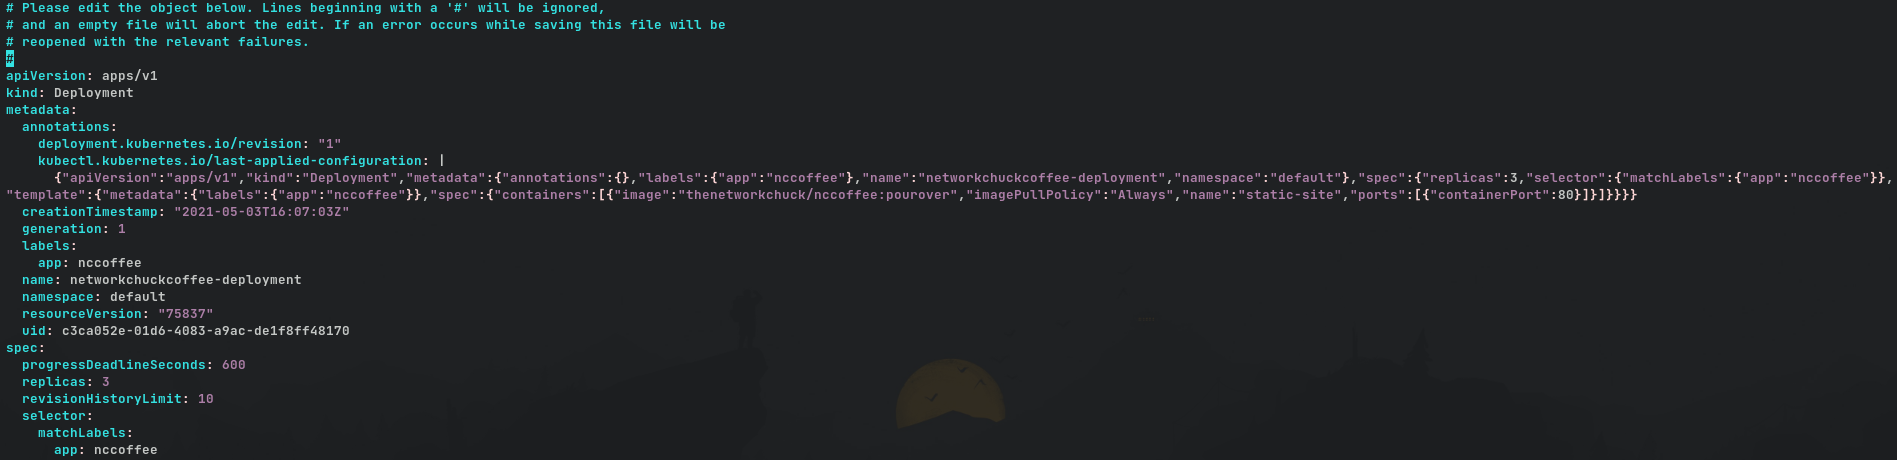
\includegraphics[width=\linewidth]{img/editDeployment1.png}
%	\caption{Output ``kubectl edit deployments'' commando}
%	\label{fig:editDeployment1}
%\end{figure}

\begin{figure}[h] 
	\inputminted[fontsize=\footnotesize,linenos]{yaml}{files/editDeployment.yaml}
	\caption{Output ``kubectl edit deployment'' commando}
	\label{editDeploy1}
\end{figure}

Als we het aantal replicas verhoogd hebben van drie naar 5 en het \verb|kubectl get pods| commando uitvoeren krijgen we, zoals in figuur \ref{fig:kubectlGetPodsEditDeploy1}, te zien dat er twee extra pods worden bijgemaakt. Deze pods worden via de ``scheduler'' op de master node verdeeld over de drie nodes in onze cluster.
\begin{figure}[h]
	\centering
	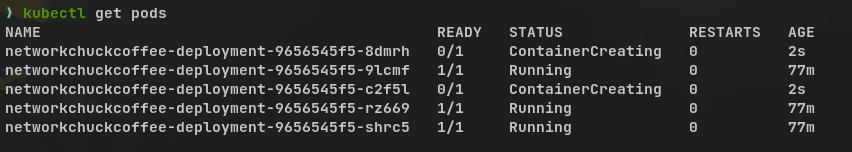
\includegraphics[width=\linewidth]{img/kubectlGetPodsEditDeploy1.png}
	\caption{Pods worden klaargemaakt}
	\label{fig:kubectlGetPodsEditDeploy1}
\end{figure}

Nu we klaar zijn met het opzetten van de deployment is het mogelijk om de cluster bloot te stellen aan het internet. Momenteel is het nog niet mogelijk om de site van buiten de cluster te bekijken. Dit komt omdat er nog geen ``service'' draait die de cluster openzet naar het internet. De service die hier zal opgezet worden zal een ``loadbalancer'' creëren op Linode die automatisch al het verkeer verdeeld over alle pods in de cluster. Het YAML bestand om de service aan te maken is te zien in figuur \ref{service1}. De code \verb|selector:app: nccoffee| zorgt ervoor dat de loadbalancer het verkeer tussen alle pods waar de applicatie ``nccoffee'' op draait verdeelt. Wanneer er pods bijkomen of verdwijnen zal de loadbalancer zich automatisch aanpassen. 

\begin{figure}[h] 
	\inputminted[fontsize=\footnotesize,linenos]{yaml}{files/testservice.yaml}
	\caption{service.yaml}
	\label{service1}
\end{figure}



Het volgend commando kan gebruikt worden om het publieke ip adres van de loadbalancer te vinden. 
\begin{minted}{bash} 
$ kubectl get services
\end{minted}

Er is ook een manier om een meer gedetailleerde beschrijving van de service te krijgen. Namelijk door middel van het volgend commando. In figuur is de output van dit commando en alle informatie over de loadbalancer service te zien. De ip adressen die worden getoond bij \verb|Endpoints:| zijn de ip adressen van alle achterliggende pods waar de ``nccoffee'' applicatie op draait. Als er nu naar het publieke ip adres van de loadbalancer wordt gesurft is de demo website te zien zoals in figuur \ref{fig:demoSite1}.
\begin{minted}{bash} 
$ kubectl describe services coffee-service 
\end{minted}

\begin{figure}[h]
	\centering
	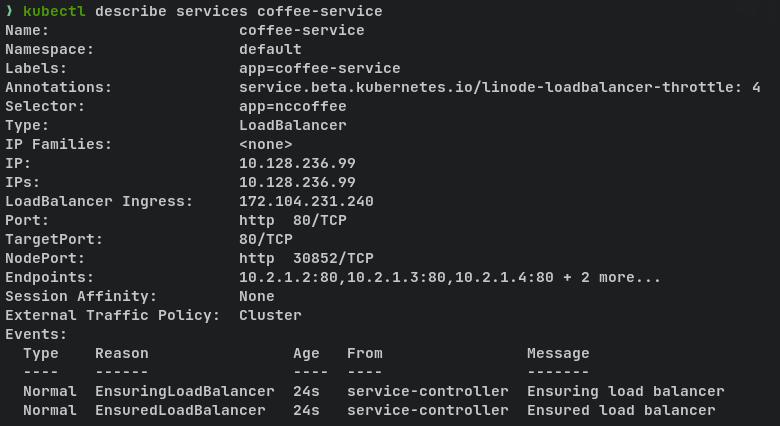
\includegraphics[width=\linewidth]{img/kubectlDescriveService1.png}
	\caption{Informatie over de loadbalancer service.}
	\label{fig:kubectlDescriveService1}
\end{figure}

\begin{figure}[h]
	\centering
	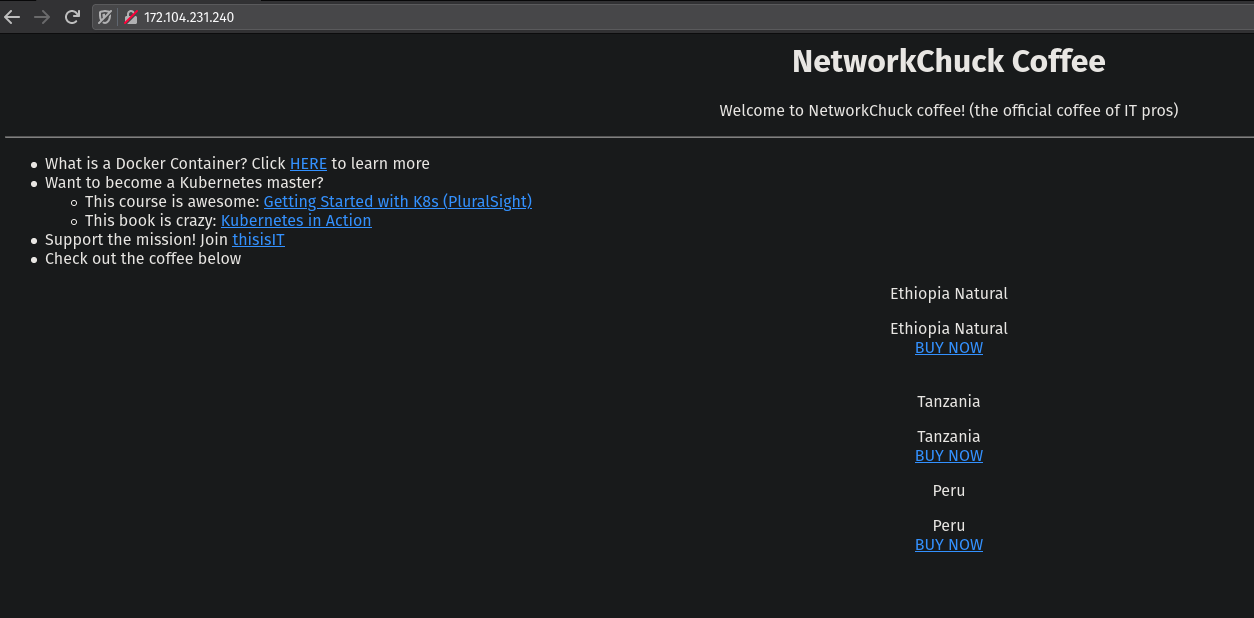
\includegraphics[width=\linewidth]{img/demoSite1.png}
	\caption{De demo website is nu zichtbaar vanop het internet.}
	\label{fig:demoSite1}
\end{figure}

\subsection{Verzamelen en analyseren van de data}

\clearpage
\section{Scenario 2: Cluster opstelling met gebruik van best practices}
\begin{itemize}
	\item Basic deployment van een statische website met best proctices uitleggen aan de hand van commando's, screenshots en config files. 
	\item Vooral RunAsUser en network policy's
	\item deployment YAML tonen en best practices uitleggen
	\item Service YAML tonen en best practices uitleggen
	\item Nodige gegevens uit de cluster halen met sysstat
	\item Verzamelde gegevens verwerken met RStudio en grafieken/statistieken tonen en uitleggen
\end{itemize}


\clearpage
\section{Scenario 3: Cluster opstelling met security tools}
\begin{itemize}
	\item Basic deployment van een statische website met enkele security tools uitleggen aan de hand van commando's, screenshots en config files. 
	\item Vooral Kubehunter en KubeBench uitleggen en praktisch voorstellen
	\item YAML files / commandos tonen en de werking uitleggen
	\item deployment YAML tonen en best practices uitleggen
	\item Service YAML tonen en best practices uitleggen
	\item Nodige gegevens uit de cluster halen met sysstat
	\item Verzamelde gegevens verwerken met RStudio en grafieken/statistieken tonen en uitleggen
\end{itemize}
